% Basic Layout settings
\documentclass[12pt]{article}
\usepackage[a4paper, margin=2.5cm]{geometry}
\usepackage[ngerman]{babel}

\usepackage{siunitx}
    \DeclareSIUnit\century{century}
    \DeclareSIUnit\year{y}

\usepackage{amsmath, amsfonts}
\usepackage{authblk}

\usepackage{enumitem}

% Section counter behavior
\usepackage{chngcntr} % Load the package for changing counter behavior

    \counterwithin{figure}{section}   % Figures numbered within sections
    \counterwithin{table}{section}    % Tables numbered within sections
    \counterwithin{equation}{section} % Equations numbered within sections

\usepackage{xcolor, cancel}

% Fonts and Colors
\usepackage[scaled]{helvet}

\renewcommand\familydefault{\sfdefault}
\usepackage{fontspec}
\usepackage[T1]{fontenc}  % T1 Font Encoding für ältere Pakete, falls erforderlich
\usepackage{titlesec}  % Paket zum Anpassen der Überschriften


\setmonofont{JetBrains Mono}[
    Path=../resources/fonts/JetBrainsMono/,
    Scale=0.85,
    Extension = .ttf,
    UprightFont=*-Regular,
    BoldFont=*-Bold,
    ItalicFont=*-Italic,
    BoldItalicFont=*-BoldItalic
]

% Farbe für den Haupttext festlegen
\usepackage{etoolbox}
\definecolor{darkgray}{gray}{0.1}
\AtBeginDocument{\color{darkgray}}

% Schriftart für die Überschriften ändern mit titlesec
\titleformat{\section}{\normalfont\sffamily\Large\bfseries\color{black}}{\thesection}{1em}{}
\titleformat{\subsection}{\normalfont\sffamily\large\bfseries\color{black}}{\thesubsection}{1em}{}
\titleformat{\subsubsection}{\normalfont\sffamily\normalsize\bfseries\color{black}}{\thesubsubsection}{1em}{}

% Anpassungen für deutsche Sprache
\addto\captionsngerman{
    \renewcommand{\figurename}{Abb.}
    \renewcommand{\listfigurename}{Abbildungsverzeichnis}
    \renewcommand{\tablename}{Tab.}
    \renewcommand{\listtablename}{Tabellenverzeichnis}
    \renewcommand{\refname}{Literaturverzeichnis}
}

\usepackage[hidelinks]{hyperref}


% Header und Footer
\usepackage{fancyhdr} % Laden des Pakets für Kopf- und Fußzeilen

\pagestyle{fancy} % Verwenden des "fancy" Stils
\fancyhf{} % Alle Kopf- und Fußzeilenfelder bereinigen
\renewcommand{\headrulewidth}{0pt} % Keine Linie im Kopfbereich
\renewcommand{\footrulewidth}{0.4pt} % Dünne Linie im Fußbereich

% Kopfzeile
\fancyhead[L]{\nouppercase{\leftmark}}
\fancyhead[C]{}
\fancyhead[R]{Stefanie Röthlisberger, Lukas Batschelet, Florian Mohaupt}

% Fußzeile
\fancyfoot[L]{}
\fancyfoot[C]{}
\fancyfoot[R]{\thepage}

% License
\usepackage[
    type={CC},
    modifier={by-nc-sa},
    version={4.0},
]{doclicense}

\usepackage{fontawesome5}

%! suppress = Makeatletter
\makeatletter
\newcommand{\github}[1]{%
    \href{#1}{\faGithubSquare}%
}
%! suppress = Makeatletter
\makeatother


% Literature management
\usepackage[backend=biber, style=apa]{biblatex}
\usepackage{graphicx}
\usepackage{float}
\addbibresource{references.bib}

% Basic document information
\title{%
    Eintwicklung eines Verfahrens zur Korngrössenanalyse mittels digitaler Höhenmodelle\\
    \normalsize Projektdokumentation}
\author[1]{Stefanie Röthlisberger}
\author[2]{Lukas Batschelet}
\author[3]{Florian Mohaupt}

\affil[1]{stefanie.roethlisberger2@students.unibe.ch, 20-924-346}
\affil[2]{lukas.batschelet@students.unibe.ch, 16-499-733}
\affil[3]{florian.mohaupt@students.unibe.ch, 22-125-041}
\date{\today}

% The Documents setup is super long and complex, therefore I decided to move it into a seperate file





\begin{document}

\maketitle

\section*{Abstract}
    In unserem Projekt haben wir die Korngrössenverteilung oberhalb des Geschiebesammlers Obermad im Gadmertal untersucht und dazu ein Programm entwickelt, welches eine Klassifikation der Korngrössenverteilung auf Basis eines digitalen Höhenmodells ermöglicht.
    Der Geschiebesammler wurde im Herbst 2023 saniert, um seine Auswirkungen auf Lebensräume, den Hochwasserschutz und den Grundwasserhaushalt zu reduzieren und einer wiederkehrenden Kiesentnahme entgegenzuwirken.

    Ursprünglich beabsichtigten wir, die Auswirkungen der Sanierungsarbeiten auf den Geschiebetransport zu analysieren.
    Da jedoch seit den Arbeiten nicht genügend Zeit verstrichen war, um eine natürlich fluvial geprägte und sortierte Umgebung wiederherzustellen, verlagerten wir unseren Fokus auf die Entwicklung eines Programms zur Klassifikation der Korngrössenverteilung.
    Dieses Verfahren nutzt digitale Höhenmodelle und ermöglicht eine effiziente und benutzungsfreundliche Analyse.

\begin{figure}[b]
    \centering
    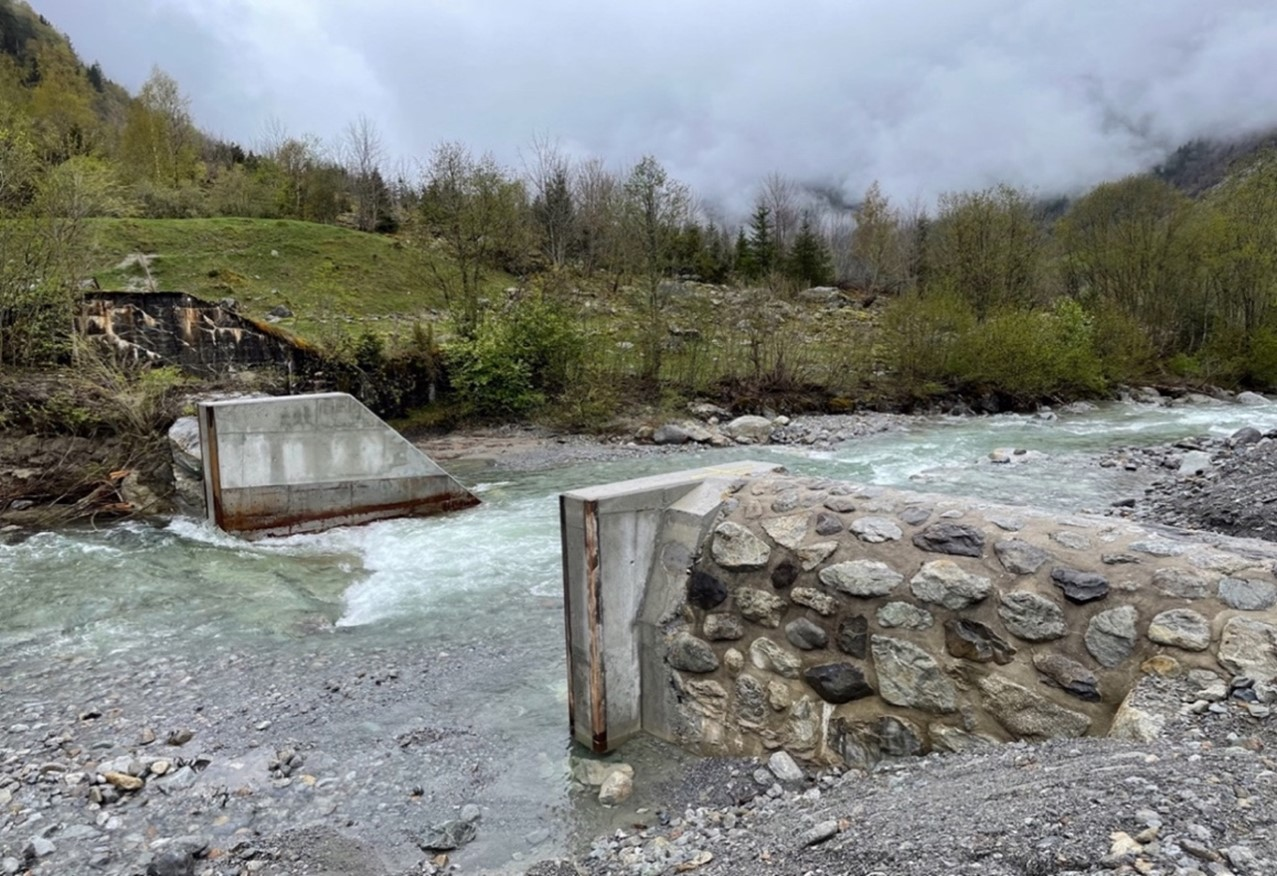
\includegraphics{../documentation/resources/images/01_titel_geschiebesammler}
    \caption{Geschiebesammler in Obermad}
    \label{fig:01_titel_geschiebesammler}
\end{figure}
\section{Einleitung}\label{sec:einleitung}

    Der Geschiebesammler Obermad wurde 2014 hinsichtlich seiner Auswirkungen auf Tiere, Pflanzen, Lebensräume, den Hochwasserschutz und den Grundwasserhaushalt untersucht.
    Die Analyse von~\cite{hunzingerGewaesserentwicklungskonzeptBernGEKOBE2014} stellte erhebliche Beeinträchtigungen in allen Bereichen fest, unter anderem aufgrund der jährlichen Entnahme von etwa 4'000 m³ Kies, woraufhin der Geschiebesammler nach Art.\ 43a GSchG als sanierungspflichtig eingestuft wurde.
    Um die negativen Effekte zu reduzieren und der wiederkehrenden Kiesentnahme entgegenzuwirken, wurde im Herbst 2023 die Durchlassbreite des Sammlers vergrössert.
    Diese Anpassung beeinflusst den Geschiebetransport und somit auch die Korngrössenverteilung des Geschiebes.
    Der natürliche Transport von Sand, Kies und Steinen im Wasser ist essenziell für die Bildung vielfältiger Strukturen im oder am Gewässer.

    Die Korngrössenverteilung spielt eine entscheidende Rolle in der Flussmorphologie und der ökologischen Dynamik von Fliessgewässern.
    Um die Korngrössen- und Geschiebeverteilung auszuwerten und zu analysieren, existieren bereits verschiedene methodische Ansätze.
    Einerseits gibt es geometrische, teils mit grossem Aufwand verbundene Verfahren, wie die Siebanalyse oder die häufiger angewendete Linienzahlanalyse~\parencite{fehrGeschiebeanalysenGebirgsflussenUmrechnung1987}.
    Bei der Linienzahlanalyse wird im Feld eine Verteilung der Komponenten manuell ausgemessen, und anschliessend wird die gesamte Korngrössenverteilung mithilfe der Fullerverteilung mathematisch angenähert~\parencite{fehrEinfacheBestimmungKorngroessenverteilung1987}.
    Nebst den geometrischen Verfahren existieren ebenfalls bereits Ansätze aus der Fotogrammmetrie, wobei anhand von hochaufgelösten Orthofotos die Geschiebeverteilung eines Gebietes analysiert werden kann.
    In junger Vergangenheit wurden auch Verfahren unter Anwendung von neuronalen Netzen für die Klassifikation entwickelt~\parencite[vgl.]{keuschSubstratkartierungAlpinenOekosystemen2023}.
    Wichtig bei solchen Verfahren ist die möglichst automatisierte und benutzungsfreundliche Anwendung, damit die entwickelten Verfahren und Methoden für verschiedene Gebiete und Fragestellungen angewendet und reproduziert werden können.

    Um eine möglichst einheitliche und nachvollziehbare Klassifikation des Geschiebehaushalts zu ermöglichen, hat das Bundesamt für Umwelt BAFU in der Vollzugshilfe zur Renaturierung von Gewässern das Substrat in fünf Klassen – Substrattypen – bezüglich Korngrösse eingeteilt.
    Es handelt sich hierbei um eine relative Klassifizierung, wobei die absoluten Korngrössen gewässerspezifisch abzuleiten sind~\parencite{nitscheGeschiebehaushaltMassnahmen2024}.
    In diesem Projekt haben wir uns bei der Klassifikation ebenfalls auf diese fünf Klassen bezogen (vgl. Abbildung 3.) % TODO: Add reference to figure

    Unser ursprüngliches Ziel war es, die Veränderungen des Geschiebetransports durch die Anpassung des Geschiebesammlers zu analysieren.
    Da jedoch nur wenige Monate zwischen der Sanierung und unseren Untersuchungen im Frühjahr 2024 lagen, war das Gebiet noch stark von der Baustelle geprägt.
    Dies führte dazu, dass sich die Umgebung noch nicht fluvial geprägt und sortiert hatte, was eine Analyse der Veränderungen der Korngrössenverteilung wenig interessant erscheinen liess.
    Aus diesem Grund fokussierten wir uns auf die Entwicklung eines datengestützten Verfahrens zur Berechnung und Kategorisierung der Korngrössenverteilung, basierend auf der Oberflächenrauheit.
    Dieses Verfahren, motiviert durch persönliches Interesse und Herausforderungen bestehender Analyseprogramme, ermöglicht eine effiziente und benutzungsfreundliche Analyse der Korngrössenverteilung.

\section{Fragestellung}\label{sec:fragestellung}

    \subsection{Forschungsfrage}\label{subsec:forschungsfrage}

    \begin{itemize}
        \item \textit{Welche Auswirkungen hat die Vergrösserung des Durchlasses des Geschiebesammlers Obermad auf die Korngrössenverteilung im Flussbett des Gadmerwasser?}
    \end{itemize}

    Die Forschungsfrage bezieht sich auf die Auswirkungen der Sanierung des Geschiebesammlers im Jahr 2023. Wir mussten im Verlauf der Arbeit feststellen, dass die effektive Beantwortung dieser Frage den Rahmen dieser Projektarbeit überschreitet. Im Abschnitt Diskussion gehen wir näher auf diese Feststellung ein. Das Ziel der Projektarbeit soll aber sein, mit der Entwicklung einer Auswertungsmethode die Beantwortung dieser Frage theoretisch zu ermöglichen.

    \subsection{Arbeitsfragen}\label{subsec:arbeitsfragen}

        Da es in dieser Arbeit vor allem darum geht, den Prozess einer fotogrammetrischen Projektarbeit kennenzulernen und selbst durchzuführen, liegt der Fokus auf den Arbeitsfragen, ohne die Forschungsfrage selbst zu beantworten.
        Unsere Hauptarbeitsfrage lautet:

        \begin{itemize}
            \item \textit{Wie kann die Oberflächenrauheit und somit die Korngrössenverteilung anhand eines digitalen Höhenmodells berechnet werden und wie lässt sich dieser Prozess vereinfachen?}
        \end{itemize}

        Zusätzlich zur oben definierten Hauptarbeitsfrage ergaben sich im Laufe des Arbeitsprozesses weitere wichtige Fragen, welche wir als Unterfragen definiert haben:

        \begin{enumerate}
            \item \textit{Wie können wir das erstellte Programm anwenden, um eine Berechnung der Korngrössen anhand der Geschiebeklassen des Bundes durchzuführen?}
            \item \textit{Wie lässt sich die entwickelte Methode zur Klassifizierung der Korngrössenverteilung auf ihre Qualität prüfen?}
        \end{enumerate}

        Für die Beantwortung dieser Arbeitsfragen entwickelten wir ein methodisches Vorgehen, welches im folgenden Kapitel näher erläutert wird.

\section{Methodisches Vorgehen}\label{sec:methodisches_vorgehen}

    Zu Beginn des Projekts haben wir verschiedene Ansätze zur Bestimmung der Korngrössenverteilung verglichen und getestet.
    Der Ansatz von Keusch (2023) ist sehr genau dokumentiert und erschien uns aufgrund der automatisierten Vorgänge zuerst vielversprechend für unser Projekt. % TODO: Add reference to Keusch
    Nach einer eingehenden Testphase stellte sich jedoch heraus, dass eine Analyse der Korngrössenverteilung mit der von Keusch vorgeschlagenen Methode von uns nicht erfolgreich umgesetzt werden konnte und den inhaltlichen und zeitlichen Rahmen dieser Projektarbeit überschreiten würde.
    Daher haben wir beschlossen, alternative Methoden zur Bestimmung der Korngrössenverteilung in Betracht zu ziehen.
    In Erwägung gezogen wurden sowohl die Nutzung von BaseGRAIN (Detert & Weitbrecht, 2013) als auch GRAINnet (Lang et al., 2021). % TODO: Add references to BaseGRAIN and GRAINnet
    Darüber hinaus bestand die Möglichkeit, ein Verfahren zu verwenden, das in der Vorlesung Geoprocessing I kurz angesprochen wurde und auf der Analyse der Oberflächenrauheit mithilfe einer überwachten Klassifikation basiert.
    Schlussendlich haben wir uns dafür entschieden, selbst eine Methode zur Analyse der Korngrössenverteilung zu entwickeln.
    Hierbei haben wir den Ansatz der Oberflächenrauheit als Mass oder Indikator für Korngrössenverteilung weiterentwickelt.

    \subsection{Programmentwicklung und -funktionen}\label{subsec:programmentwicklung-und--funktionen}

        Das GeoRoughness Tool ist ein selbst entwickeltes Software-Tool zur Analyse digitaler Höhenmodelle (DEMs), welches die Korngrössenverteilung innerhalb quadratischer Untersuchungsfenster berechnet.
        Die Software bietet ein einfaches grafisches User Interface (GUI), was die Anwendung benutzungsfreundlich gestaltet. 
        Das Programm wurde in Python geschrieben, weil Python diverse Libraries für das Arbeiten mit räumlichen Daten bietet. 
        Wir verwenden die Rasterio\footnote{\href{https://rasterio.readthedocs.io/en/stable/}{https://rasterio.readthedocs.io/en/stable/}} Library, welche gut geeignet ist für Berechnungen mit Rasterdateien.
        Das Programm ist als Python Package verfügbar und läuft unabhängig vom vorhandenen Betriebssystem auf allen Computern, welche mindestens Python 3.12 installiert haben.\footnote{Detaillierte Anleitung zur Installation unter \href{https://github.com/lbatschelet/GeoRoughness-Tool}{https://github.com/lbatschelet/GeoRoughness\-Tool}}

        Für die Berechnung und Kategorisierung der Korngrössenverteilung verwenden wir die Oberflächenrauheit als Proxy, unter der Annahme, dass eine grosse Oberflächenrauheit mit grossen Korngrössen einhergeht.
        Rauheit bezieht sich im Zusammenhang mit Digitalen Höhenmodellen (DEM) auf die Variabilität oder Unregelmässigkeit der Höhenwerte innerhalb eines bestimmten Gebietes und wird deshalb häufig mit der Standardabweichung der Höhenwerte ausgedrückt.
        Die Standardabweichung ist ein Mass für die Schwankung oder Streuung einer Gruppe von Werten.
        Sie wird als die Quadratwurzel der Varianz berechnet (vgl. \ref{eq:standardabweichung}).
        Die Grösse des gewählten Bereichs beeinflusst die Rauheitsberechnung, wobei kleinere Fenster lokale Abweichungen stärker hervorheben und grössere Fenster lokale Abweichungen glätten.

        \begin{equation}
            \sigma = \sqrt{\frac{1}{N} \sum_{i=1}^{N} (x_i - \mu)^2}
            \label{eq:standardabweichung}
        \end{equation}

        Da die Berechnung von diversen Bedingungen, wie bspw.\ der räumlichen Auflösung des zur Verfügung stehenden DEM, abhängt und entscheidend beeinflusst werden kann, bietet das Tool mehrere Parameter (vgl.\ Abbildung 5), um mit verschiedenen Datensätzen umgehen zu können. 
        Wir wollen hier die zwei wichtigsten Parameter kurz vorstellen, eine ausführlichere Dokumentation aller Parameter ist im Projektwiki auf GitHub\footnote{\href{https://github.com/lbatschelet/GeoRoughness-Tool/wiki/Parameter-Explanation}{https://github.com/lbatschelet/GeoRoughness\-Tool/wiki/Parameter\-Explanation}} abgelegt.

        Der Window Size Parameter bestimmt die Seitenlänge des quadratischen Untersuchungsfensters, bestimmt also die Grösse der Pixel in der Ausgabedatei.
        Der Wert kann als positive, rationale Zahl in Metern eingegeben werden.
        Standardwert ist 1.0 Meter. % TODO: format

        Kommagetrennte Schwellenwerte (Categorical Thresholds) ermöglichen es die Korngrössenverteilung in diskrete Klassen einzuteilen.
        Dadurch werden nummerierte Kategorien erstellt, die durch die angegebenen Schwellenwerte getrennt sind.
        Mithilfe dieser Funktion haben wir unser Resultat in die fünf Korngrössenklassen eingeteilt.
        Die tatsächlichen Schwellenwerte werden sich von Projekt zu Projekt vermutlich stark verändern, da sie von der berechneten Oberflächenrauheit abhängen.
        Diese ist wiederum stark abhängig von der räumlichen Auflösung des zugrunde liegenden DEM.
        Um die Korngrössenverteilung in $n$ Klassen einzuteilen werden $n+1$ kommagetrennte, positive und rationale Schwellenwerte benötigt.
        Dies da unterhalb des tiefsten Schwellenwertes eine Kategorie 0 (für flache Regionen wie betonierte Plätze) und oberhalb des obersten Wertes eine höchste Kategorie (für Ausreisser und Extremwerte) hinzugefügt wird.

        \begin{minipage}{.45\textwidth}
            \begin{figure}[H]
                \centering
                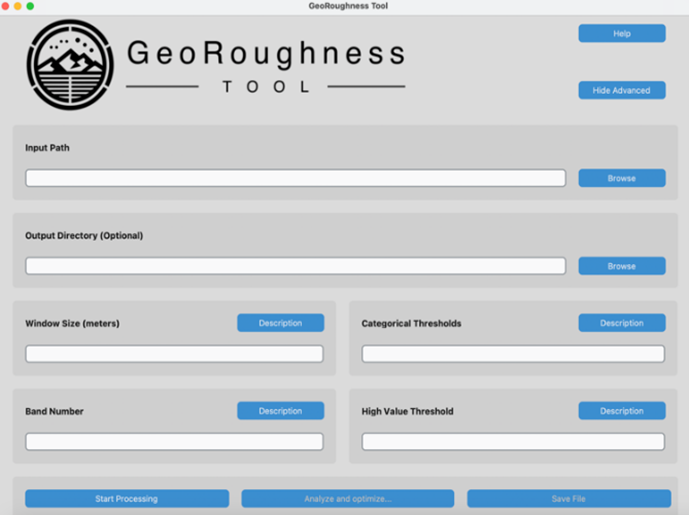
\includegraphics[width=\linewidth]{C:\Users\batsc\IdeaProjects\GeoRoughness-Tool\documentation\resources\images\05_Programm_Oben}
                \caption{Grafische Benutzeroberfläche (GUI) vom GeoRoughness-Tool}
                \label{fig:05_programm_oben}
            \end{figure}
        \end{minipage}
        \hfill
        \begin{minipage}{.45\textwidth}
            \begin{figure}[H]
                \centering
                \includegraphics[width=\linewidth]{C:\Users\batsc\IdeaProjects\GeoRoughness-Tool\documentation\resources\images\06_Programm_Unten}
                \caption{Pseudogefärbte Klassifizierung der Oberflächenrauheit im GUI}
                \label{fig:06_programm_unten}
            \end{figure}
        \end{minipage}

        Um die Qualität der allfällig gewählten Schwellenwerte zu überprüfen, kann nach einer ersten Berechnung ein Vergleich der berechneten Werte mit einer Trainingsdatei durchgeführt werden (vgl. Kapitel 3.3.2.) % TODO: Add reference to chapter 3.3.2
        Dies geschieht mit der Funktion Analyze and Optimize (vgl.\ Abbildung 7). % TODO: Add reference to figure
        Dort kann die Trainingsdatei eingeladen werden, um anschliessend optimierte Schwellenwerte zu berechnen.

        Um die optimierten Schwellenwerte zu berechnen, iteriert das Programm über jede Kategorie aus den Trainingsdaten und sammelt für jedes Pixel aus der entsprechenden Kategorie die ursprünglichen Oberflächenrauheit.
        Daraus entsteht für jede Kategorie eine Liste mit den darin enthaltenen Oberflächenrauheitswerten.
        Da die Kategorisierung der Trainingsdaten visuell erfolgt und nicht basierend auf den berechneten Werten, ist damit zu rechnen, dass sich die Kategorien nicht klar voneinander trennen werden und überschneiden.
        Deshalb berechnet das Programm den tatsächlichen Schwellenwert zwischen zwei Kategorien durch den Mittelwert des 95 Perzentil der unteren, und des 5 Perzentil der oberen Kategorie.
        Die Berechnung des untersten und des obersten Schwellenwertes erfolgt leicht anders, so sollen alle Werte der Trainingsdaten hier erhalten bleiben, zudem wird sichergestellt, dass der tiefste Schwellenwert immer grösser als 0 ist.
        Diese optimierten Schwellenwerte können kopiert und bei Categorical Thresholds wiederum eingefügt werden, um eine optimierte Klassifikation zu erhalten.


        Auf den aktuellen Entwicklungsstand sowie mögliche Erweiterungen gehen wir in Kapitel 5.1 ein. % TODO: Add reference to chapter 5.1

        \begin{figure}
            \centering
            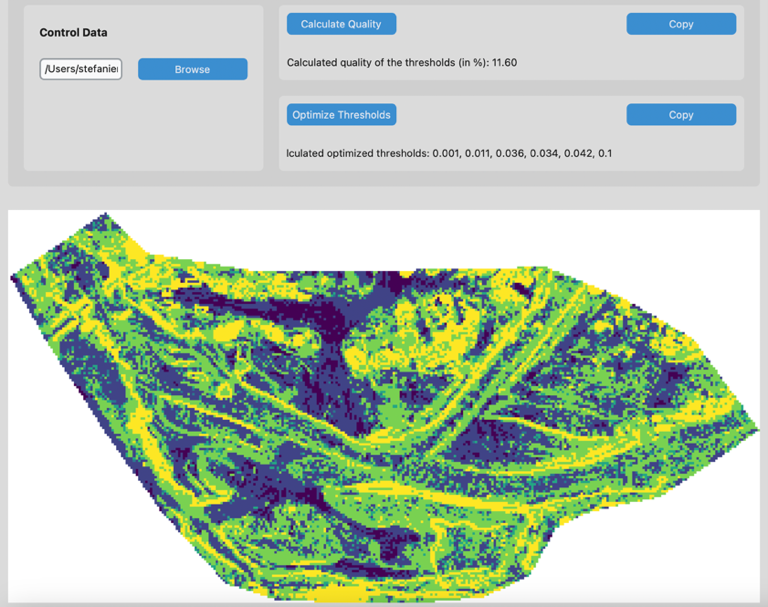
\includegraphics[width=0.5\linewidth]{C:\Users\batsc\IdeaProjects\GeoRoughness-Tool\documentation\resources\images\07_threshold_optimizer}
            \caption{Optimierung der Thresholds}
            \label{fig:07_threshold_optimizer}
        \end{figure}

    \subsection{Feldarbeit}\label{subsec:feldarbeit}

        Um aktuelle Daten für die anschliessende Analyse zu erhalten, wurde eine fotogrammetrische Vermessung des Untersuchungsgebiets durchgeführt.
        Die Feldarbeit in Obermad umfasste das Festlegen und Vermessen der Ground Control Points (GCPs), sowie eine Befliegung des gesamten Untersuchungsgebiets mit einer Drohne, um Luftbilder aufzunehmen.

        Um qualitativ hochwertige Bildaufnahmen zu erstellen, sollte die Befliegung an einem Tag mit minimalem oder keinem Niederschlag durchgeführt werden.
        Bei der Feldmessungen am 08.\ Mai 2024 trat leichter Nieselregen auf, was jedoch die Qualität der erhobenen Daten nicht beeinträchtigte.
        Ein potenzielles Problem hätten kleine Wassertropfen auf der Kameralinse darstellen können.
        Durch das stetige Abwärtsrichten der Kamera konnte dieses Risiko minimiert werden.

        Nach einer kurzen Begehung des Untersuchungsgebiets begann die Feldarbeit mit dem Setzen der GCPs.
        Dafür wurden 10 gut sichtbare Kreuze aus gelbem Klebeband (vgl.\ Abbildung 9) gleichmässig im gesamten Untersuchungsgebiet verteilt. % TODO: Add reference
        Eine, wegen einem niederschlagsreichen Frühling zusätzliche Herausforderung bestand darin, die GCPs auf der anderen Seite des Flusses zu verteillen.
        Anschliessend wurden alle gesetzten GCPs mithilfe eines GNSS-Empfängers vermessen (vgl. Abbildung 10.) % TODO: Add reference
        GNSS ermöglicht die schnelle und genaue Bestimmung der absoluten Positionskoordinaten der Punkte und gewährleistet eine unabhängige Kontrolle.
        Bei der Messung im Feld wurden kontinuierlich Signale von ungefähr 15 bis 20 Satelliten empfangen, was eine sehr genaue Positionierung ermöglichte.
        Die hohe Anzahl an Empfangssignalen reduzierte den Effekt der Dilution of Precision (DOP).
        Dieser Effekt kann durch eine verteilte Anordnung der sichtbaren Satelliten im Orbit verkleinert werden, sodass die Genauigkeit der Messung weniger stark beeinflusst wird.

        \begin{figure}
            \centering
            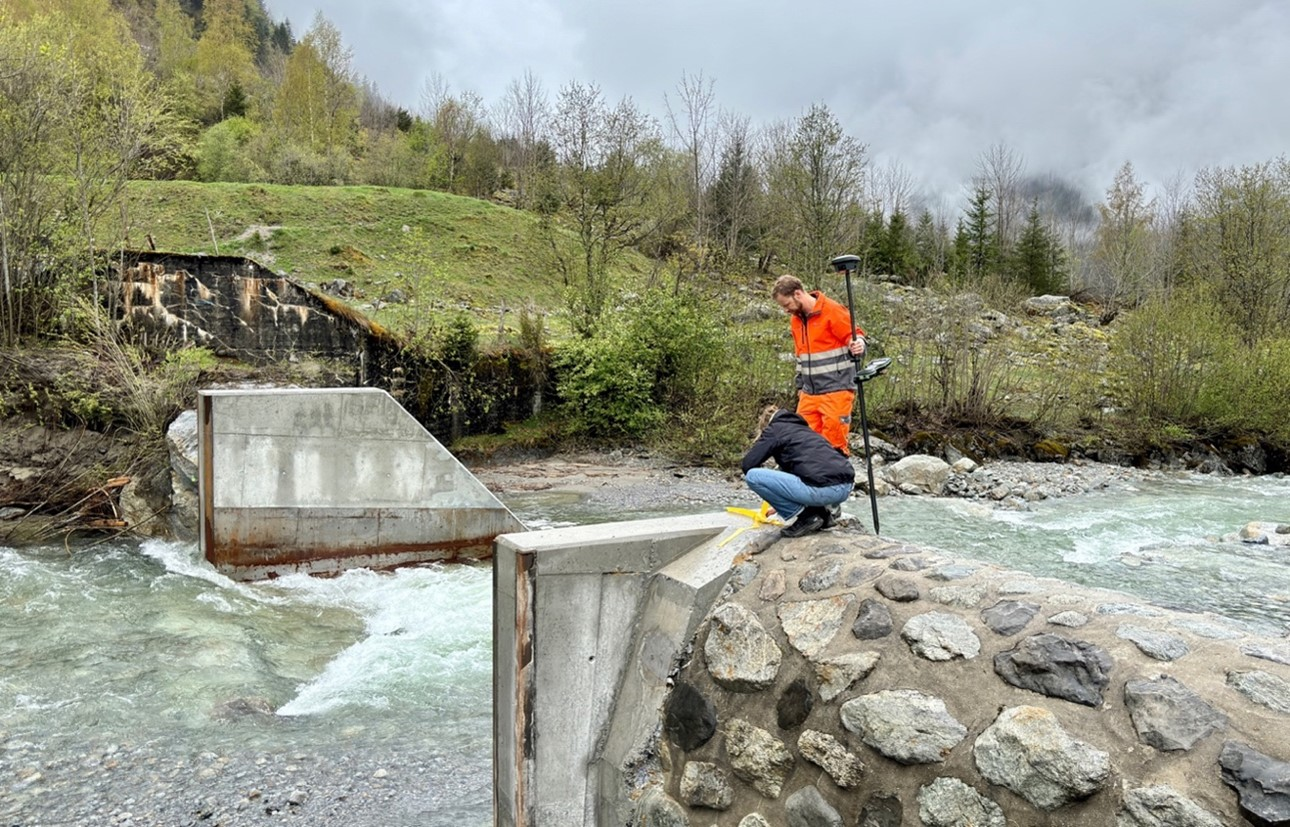
\includegraphics{C:\Users\batsc\IdeaProjects\GeoRoughness-Tool\documentation\resources\images\08_GCPs_setzen}
            \caption{Definieren und Vermessen eines GCPs auf dem Geschiebesammler}
            \label{fig:08_gcps_setzen}
        \end{figure}

        \begin{minipage}{.45\textwidth}
            \begin{figure}
                \centering
                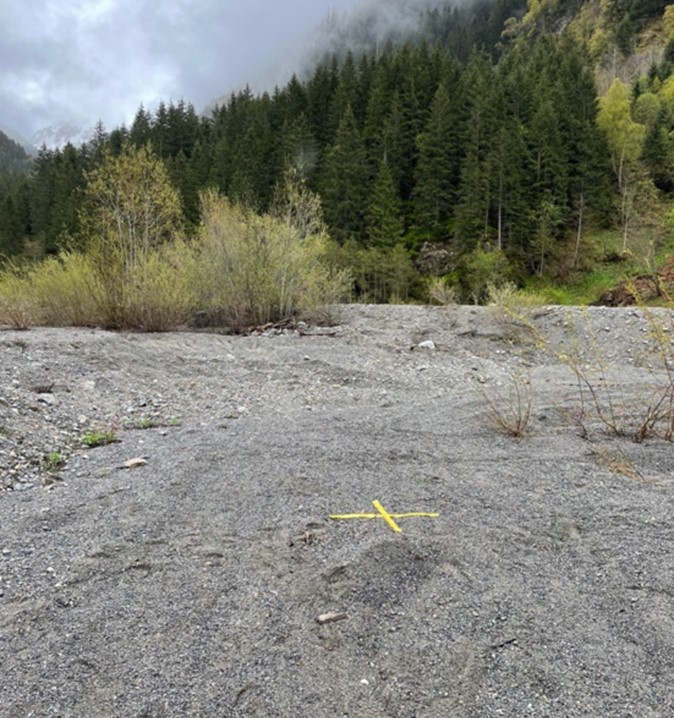
\includegraphics[width=\linewidth]{C:\Users\batsc\IdeaProjects\GeoRoughness-Tool\documentation\resources\images\09_GCP}
                \caption{GCP-Markierung (eigene Aufnahme)}
                \label{fig:09_gcp}
            \end{figure}
        \end{minipage}
        \hfill
        \begin{minipage}{.45\textwidth}
            \begin{figure}
                \centering
                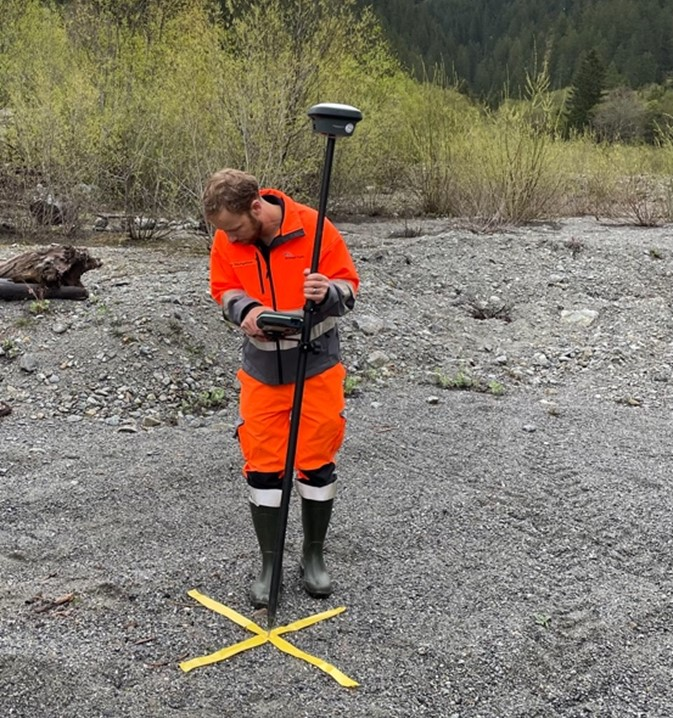
\includegraphics[width=\linewidth]{C:\Users\batsc\IdeaProjects\GeoRoughness-Tool\documentation\resources\images\10_GCP_GNSS_Vermessung}
                \caption{GNSS-Vermessung (eigene Aufnahme)}
                \label{fig:10_gcp_gnss_vermessung}
            \end{figure}
        \end{minipage}

        Vor der Befliegung des gesamten Untersuchungsgebiets mit der Drohne mussten wir uns überlegen, welche Auflösung, Flughöhe und welcher Ausschnitt für unser Projekt geeignet ist.
        Da das Untersuchungsgebiet in Obermad bereits mehrmals beflogen wurde, war dieses bereits vordefiniert.
        Wie in Abbildung 11 zu sehen, wurden uns Orthofotos von früheren Befliegungen von der Kraftwerke Oberhasli AG zur Verfügung gestellt, die wir als Referenzrahmen für Auflösung und Flughöhe nutzten. % TODO: Add reference
        Die Auflösung liegt bei 0.02 Meter mit einer Flughöhe von ungefähr 40 Metern.

        \begin{figure}
            \centering
            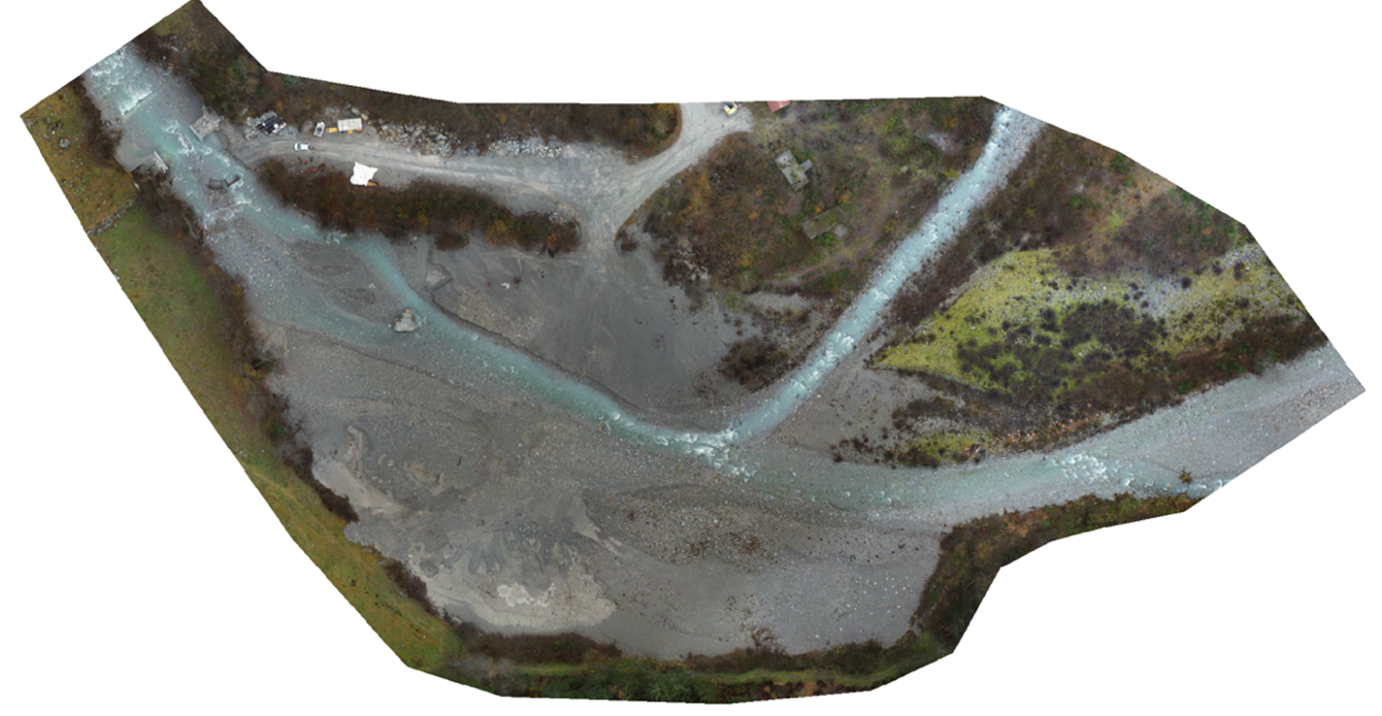
\includegraphics{C:\Users\batsc\IdeaProjects\GeoRoughness-Tool\documentation\resources\images\11_Orthofoto}
            \caption{Orthofoto vom 16.11.2023 als Referenz für Grösse des Untersuchungsperimeters.}
            \label{fig:11_orthofoto}
        \end{figure}

        Für die Befliegung kam eine DJI Matrice 300 RTK-Drohne zum Einsatz, auf welcher eine DJI Zenmuse P1 Kamera installiert war.
        Die Drohne verwendet das Echtzeitkinematik-Verfahren (RTK), welches eine sehr genaue Positionierung mithilfe von GNSS und zusätzlichen Boden-Referenzpunkten ermöglicht.
        Der Drohnenflug wurde von Jan Baumgartner durchgeführt.
        Hierbei war es wichtig, dass wir die Drohne immer im Sichtfeld behielten, um sie bei allfällig auftauchenden Problemen lokalisieren zu können.
        Der gesamte Perimeter wurde mit hohem Überschneidungsgrad abgeflogen, damit Lücken in der Punktwolke möglichst vermieden werden können.

        \begin{minipage}{.45\textwidth}
            \begin{figure}
                \centering
                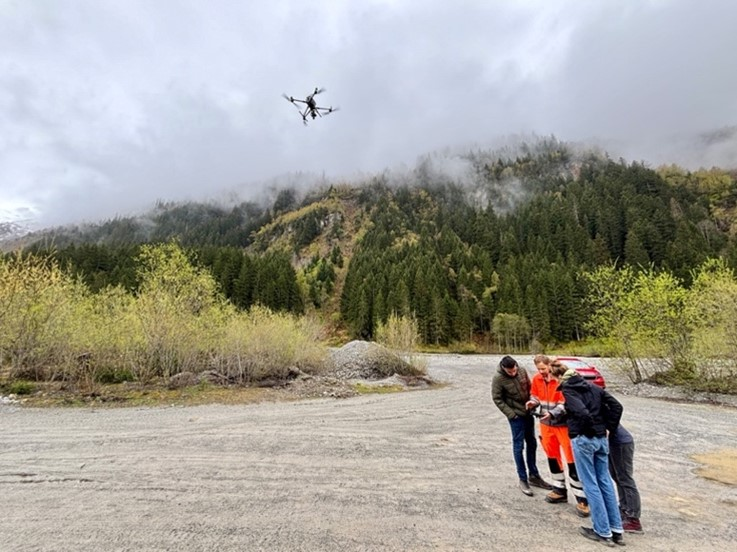
\includegraphics[width=\linewidth]{C:\Users\batsc\IdeaProjects\GeoRoughness-Tool\documentation\resources\images\12_Befliegung}
                \caption{Befliegen des Untersuchungsperimeters (eigene Aufnahme)}
                \label{fig:12_befliegung}
            \end{figure}
        \end{minipage}
        \hfill
        \begin{minipage}{.45\textwidth}
            \begin{figure}
                \centering
                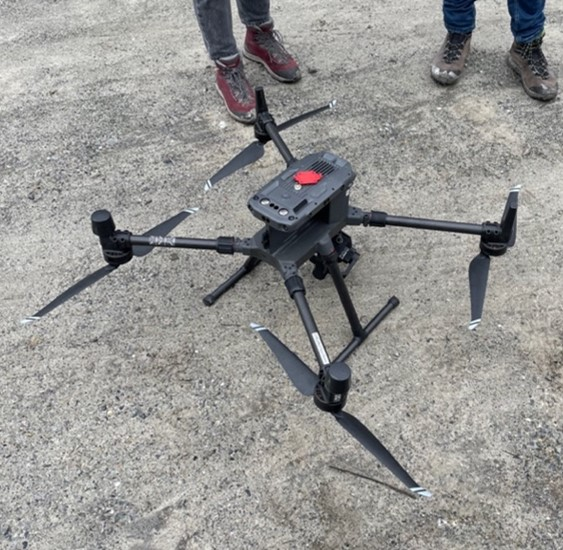
\includegraphics[width=\linewidth]{C:\Users\batsc\IdeaProjects\GeoRoughness-Tool\documentation\resources\images\13_Drohne}
                \caption{DJI Matrice 300 RTK mit DJI Zenmuse P1 (eigene Aufnahme)}
                \label{fig:13_drohne}
            \end{figure}
        \end{minipage}

        Direkt nach der Befliegung haben die Daten auf einem PC gesichert.
        Noch im Feld erstellten wir in Agisoft Metashape aus den gewonnenen Daten eine dünn besetzte Punktwolke (vgl.\ Abbildung 14) , um die Überschneidung und somit mögliche Lücken zu identifizieren.
        Falls hierbei grössere Lücken aufgefallen wären, hätten wir eine zweite Befliegung durchgeführt.
        Nachdem wir die Daten zusätzlich in der Cloud gesichert hatten, war die Arbeit im Feld abgeschlossen und wir hatten alle nötigen Daten, um mit dem Post-Processing zu beginnen.

        \begin{figure}
            \centering
            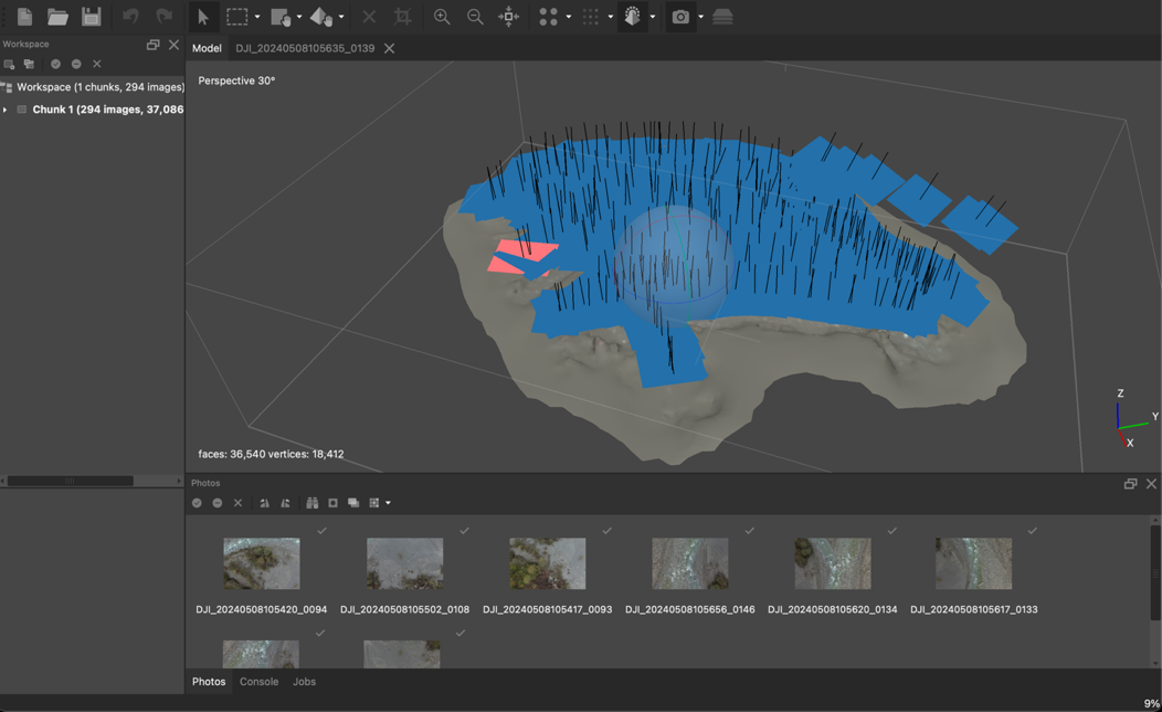
\includegraphics{C:\Users\batsc\IdeaProjects\GeoRoughness-Tool\documentation\resources\images\14_Agisoft}
            \caption{Die Bilder wurden noch im Feld auf Lücken geprüft}
            \label{fig:14_agisoft}
        \end{figure}

    \subsection{Post-Processing}\label{subsec:post-processing}
        Im Post-Processing ging es darum, die aufgenommenen Luftbilder weiterzuverarbeiten, damit das erstellte Höhenmodell mithilfe des entwickelten Tools analysiert werden konnte. 
        Wichtig war am Schluss die Überprüfung der automatisierten Klassifikation mithilfe des visuell definierten Testgebiets. 
        In den folgenden Unterkapiteln wird durch den typischen Workflow einer Anwendung des GeoRoughness Tools geführt.

        \subsubsection{Erstellung Höhenmodell und Orthofoto}\label{subsubsec:erstellung-hoehenmodell-und-orthofoto}

            Hierfür wurde das Programm \textit{Agisoft Metashape Professional} verwendet.
            Mit dem Programm können 3D-Modelle, Höhenmodelle und Orthofotos aus Luftbildaufnahmen erzeugt werden.
            Damit dieser Arbeitsschritt korrekt durchgeführt werden kann, ist es wichtig, dass die Luftbilder eine genügend hohe Überschneidung – ungefähr 60 \% in alle Richtungen – aufweisen (Kraftwerke Oberhasli AG, 2022). % TODO: Add citation
            In dieser Arbeit wird auf eine detaillierte Beschreibung der nötigen Arbeitsschritte verzichtet, da eine Anleitung im Rahmen der Vorlesung zur Verfügung gestellt wurde.
            Ein wichtiger Schritt für ein qualitativ hochwertiges Endprodukt war das Verknüpfen der ausgemessenen Koordinaten der GCPs mit der Punktewolke.
            Als Endprodukte des gesamten Arbeitsschritts liegen ein Orthofoto sowie das Höhenmodell (DEM) in Form von .tiff-Dateien vor. % TODO format

        \subsubsection{Definition von einem Trainingsgebiet in QGIS}\label{subsubsec:definition-von-einem-trainingsgebiet-in-qgis}

            Zur Optimierung der Grenzwerte für die Klassifikation der Rauheitsklassen haben wir in einem ersten Schritt ein Trainingsgebiet manuell zugewiesen.
            Dieses Trainingsgebiet dient dazu, optimierte Grenzwerte zu berechnen, die anschliessend auf das gesamte Untersuchungsgebiet angewendet werden können.

            \begin{figure}
                \centering
                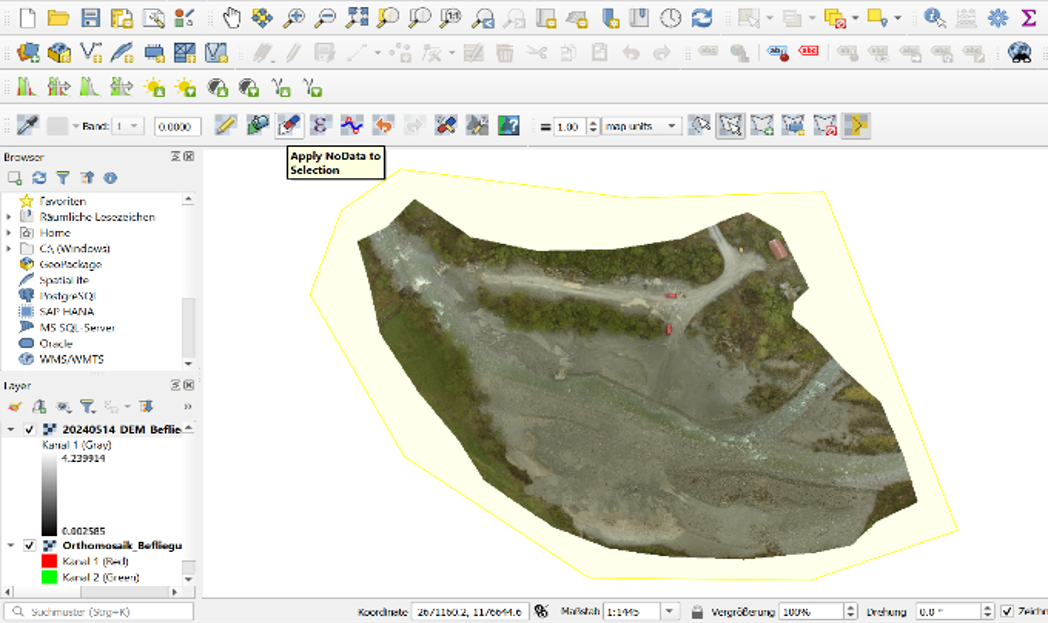
\includegraphics{C:\Users\batsc\IdeaProjects\GeoRoughness-Tool\documentation\resources\images\15_NoData_setzen}
                \caption{Rasterwerte mit dem Serval Plugin auf NoData setzten}
                \label{fig:15_nodata_setzen}
            \end{figure}

            Um die Datei für die manuelle Klassifizierung vorzubereiten, haben wir uns vom Tool zunächst eine Datei mit willkürlich gesetzten Grenzwerten erstellen lassen.
            Diese Datei hatte dann bereits die passende Pixelgrösse.
            Anschliessend luden wir diese Datei zusammen mit dem zuvor erstellten Orthofoto in QGIS.
            Mit dem QGIS-Plugin \textit{Serval}\footnote{\href{https://plugins.qgis.org/plugins/Serval/}{https://plugins.qgis.org/plugins/Serval/}} setzten wir alle Pixelwerte (vgl. Abbildung 15) in der vorläufig kategorisierten Datei auf NoData (Serval → Select Raster cells by Polygon → Apply NoData to Selection). % TODO: Add reference to figure

            Auf dem Orthofoto suchten wir dann ein Gebiet, in dem alle Korngrössenklassen mehrfach vertreten sind. 
            Wir entschieden uns für ein Gebiet von 14 x 14 Metern (vgl. Abbildung 16). % TODO link
            Obwohl das Tool keine Mindestgrösse für das Trainingsgebiet festlegt, verbessert ein grösseres Gebiet tendenziell die Qualität des Endprodukts.
            
            Die Kategorisierung führten wir auf Basis der Vollzugshilfe für Massnahmen zum Geschiebehaushalt des Bundesamtes für Umwelt durch (Nitsche & Pfaundler, 2024). % TODO reference
            Jedem Pixel in der nun leeren Datei wiesen wir visuell einen Wert von 1 bis 5 zu (Serval → Apply Value to single cell), entsprechend der vorgesehenen Kategorie.
            Diese visuelle Zuweisung ist stark abhängig von der einschätzenden Person und stellt eine potenzielle Fehlerquelle dar.
            Herausforderungen, wie beispielsweise das Vorhandensein eines grossen Steins in überwiegend feinkörnigem Geschiebe, bei dem keine Kategorie wirklich passte, werden detailliert in Kapitel 5 behandelt. % TODO link

            \begin{figure}
                \centering
                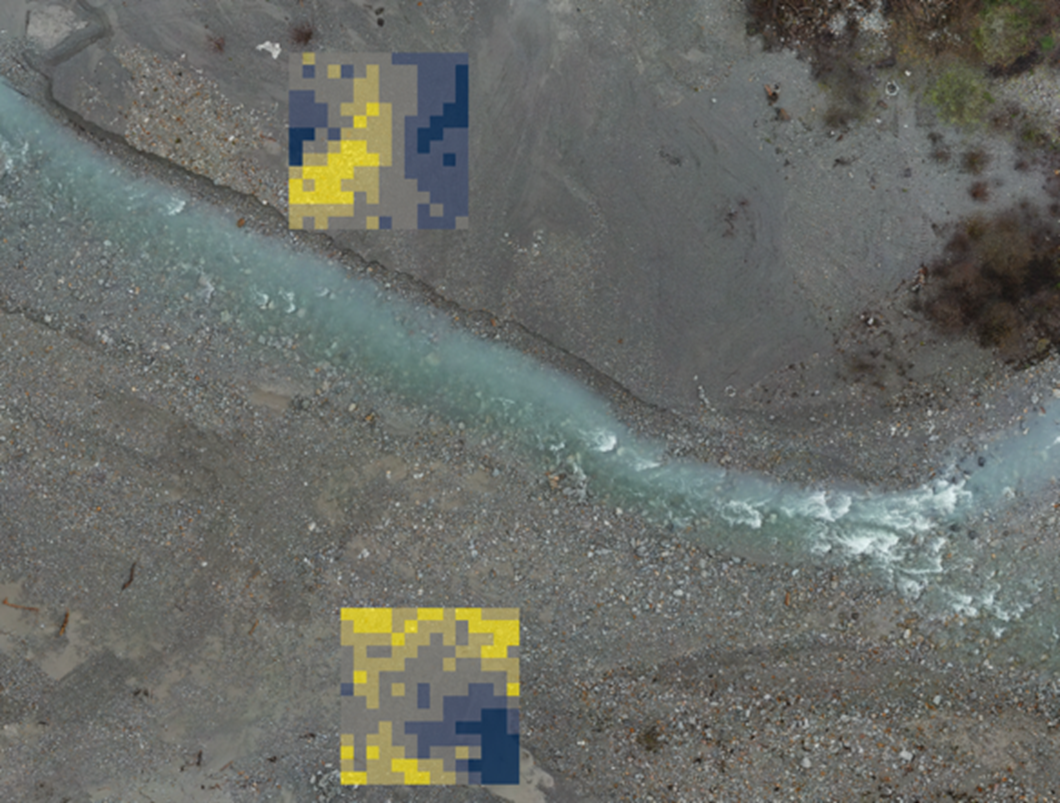
\includegraphics{C:\Users\batsc\IdeaProjects\GeoRoughness-Tool\documentation\resources\images\16_Trainingsgebiet}
                \caption{Trainingsgebiet (oben) und das im Kapitel 3.4 zur Validierung erstellte Testgebiet (unten) über dem Orthofoto.}
                \label{fig:16_trainingsgebiet}
            \end{figure}

        \subsubsection{Datenauswertung im GeoRoughness Tool}\label{subsubsec:datenauswertung-im-georoughness-tool}

            Die in Kapitel 3.3.2 erstellten Trainingsdaten können nun in einem nächsten Schritt mit Hilfe der Funktion Analyze and Optimize zurück in das Tool geladen werden. % TODO link
            Dort haben wir mit den Trainingsdaten optimierte Grenzwerte berechnet. 
            Die berechneten Grenzwerte können dann wiederum verwendet werden um die Kategorisierung auf die ganze Datei anzuwenden. 
            Das Tool liefert nun eine zweite Datei mit den angepassten Kategorien. 
            Mit diesem Vorgehen können grosse Gebiete in kurzer Zeit automatisch kategorisiert werden.

    \subsection{Überprüfung der Methode}\label{subsec:ueberpruefung-der-methode}
        Um die entwickelte Methode überprüfen zu können wurde im gleichen Untersuchungsgebiet wie im Kapitel 3.3 ein zusätzliches Testgebiet ausgewiesen. % TODO link
        Das Vorgehen dafür ist identisch wie im Kapitel 3.3.2. % TODO link

        Um die Qualität der Methode festzustellen, wurde die berechnete Klassifizierung mit dem Testgebiet verglichen.
        Dafür musste der ebenfalls 14 x 14 Pixel grosse Testbereich extrahiert werden, da nur in diesem Bereich die Abweichungen bestimmt wurden.
        Danach wurde in QGIS mithilfe des Raster Calculators die Differenzen zwischen den beiden Layer berechnet und anschliessend in einem neuen Layer abgespeichert.

        Die Abweichungen von den Testklassen zu den automatisch kategorisierten Klassen konnten die Werte -5 bis +5 annehmen.
        Ein Wert von 0 ist optimal, was bedeutet, dass die entwickelte Methode das Pixel in die genau gleiche Rauheitskategorie eingeteilt hat, wie bei der visuell vorgenommenen Kategorisierung.
        Eine gewisse Abweichung ist von Abbildung 17 zu Abbildung 18 bereits von Auge erkennbar, diese ist zu gewissem Teil auf die subjektive visuelle Einteilung der Trainings- und Testdaten zurückzuführen. % TODO link
        Die absoluten Differenzen zwischen dem Testgebiet und der automatisch berechneten Rauheit sind in Abbildung 19 sichtbar. % TODO link
        Genauer besprochen werden die Resultate im nächsten Kapitel.

        \begin{figure}
            \centering
            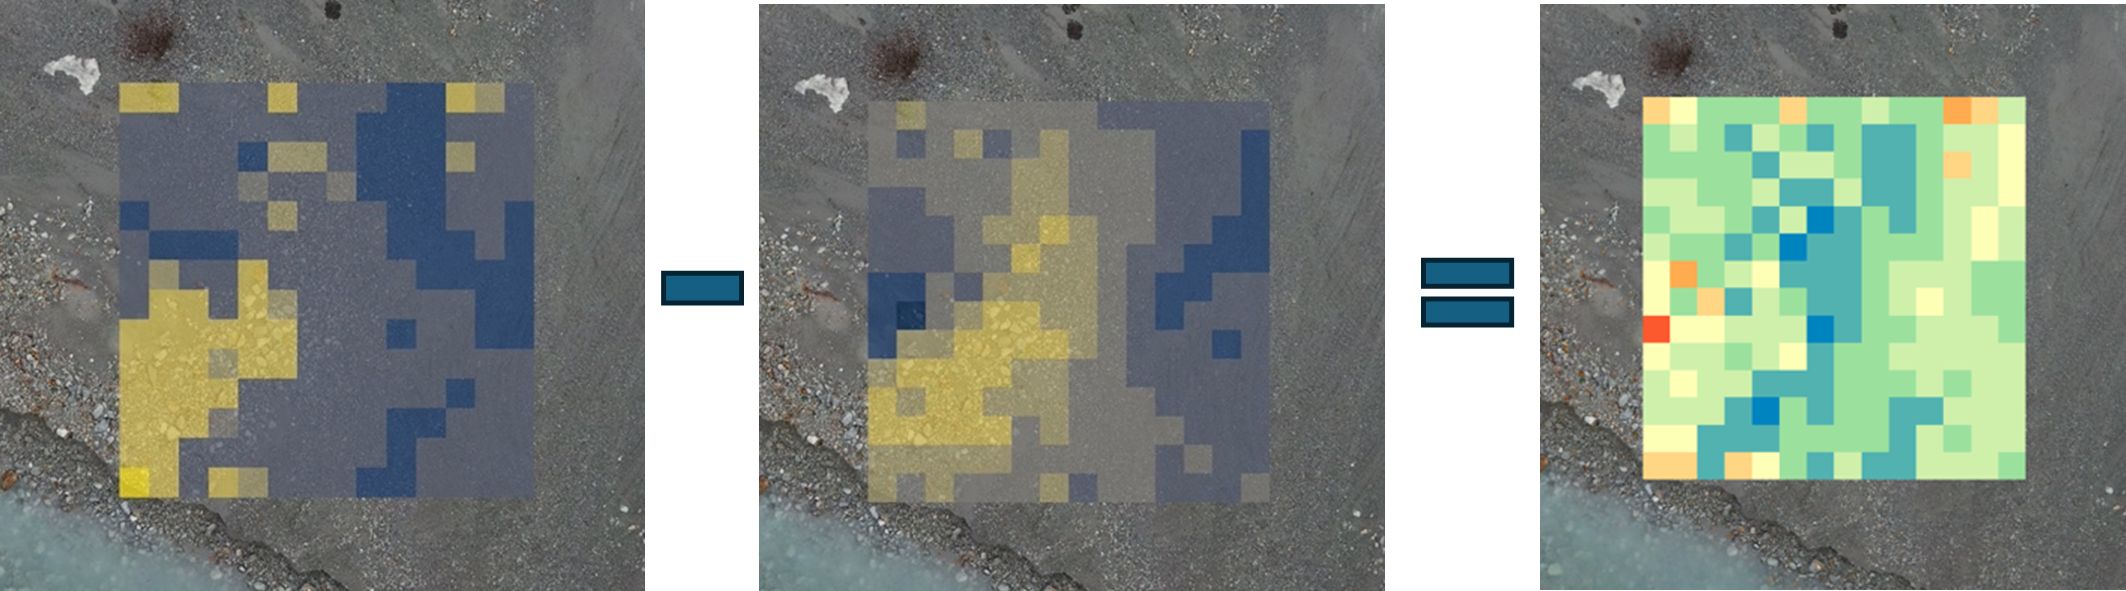
\includegraphics{C:\Users\batsc\IdeaProjects\GeoRoughness-Tool\documentation\resources\images\zusammengesetzte_abbildungen}
            \caption{Automatisch generierte Klassifizierung (links), Visuelle Klassifizierung (mitte), Differenz wobei eine grosse Differenz dunkel, und eine kleine Differenz hell dargestellt wird (rechts)}
            \label{fig:zusammengesetzte_abbildungen}
        \end{figure}

\section{Resultate}\label{sec:resultate}

    Mit einer statistischen Analyse in Excel ist es möglich, die Zuverlässigkeit und Präzision des entwickelten GeoRoughness Tools zu überprüfen.
    Hierfür wurde ein Histogramm (vgl. Abbildung 20) erstellt, in welchem die Differenz zwischen den automatisch berechneten Substratklassen und den visuell kategorisierten Klassen im Kontrollgebiet ersichtlich wird. % TODO link
    Mit einem Mittelwert von - 0.52 ist ein Negativ-Trend sichtbar, was bedeutet, dass die Kontrolldaten tendenziell in höhere (gröbere) Substratklassen eingeteilt wurden als vom Programm selbst.
    Hierbei muss erwähnt werden, dass sich die visuelle Einteilung teils schwierig gestaltete, da die Substratklassen von mehrheitlich einheitlicher Substratverteilung pro Pixel ausgehen, dies jedoch nicht immer der Fall war.
    Wenn beispielsweise ein grösserer Stein inmitten von sehr feinkörnigen Sedimentablagerungen lag, war die Klasseneinteilung unklar und deshalb wohl nicht immer ähnlich wie die des GeoRoughness Tools, welches die Einteilung statistisch nach Höhenunterschieden und anhand der Trainingsdaten durchführt, was sich auf die Resultate auswirken kann.
    Ebenfalls haben die gewählten Thresholds einen Einfluss auf die Resultate.
    Die vom Programm als optimale Thresholds berechneten Werte für die Substratklassen, welche für das Endprodukt genutzt wurden, waren folgende: 0.001, 0.011, 0.034, 0.036, 0.042, 0.142.

    Mit dem Endresultat sind wir zufrieden, da der Grossteil der Pixel korrekt oder nur mit einer Abweichung von 1 klassiert wurde. 
    Dies deutet darauf hin, dass das entwickelte Programm funktioniert und für Rauheitsklassifikationen angewendet werden kann. 
    Das Resultat ist jedoch stark abhängig von den verwendeten Trainingsdaten, weshalb eine sorgfältige Klassifikation dieser sehr wichtig ist. 
    Die benutzten Thresholds können je nach Trainingsdaten variieren, weshalb bei einem grösseren Zeitrahmen des Projekts sicher ein mehrmaliger Durchlauf des Programms mit mehreren Trainingsdaten oder grösseren Trainingsgebieten empfehlenswert ist, um aussagekräftige Resultate zu erhalten.
    
    Nebst dem Resultat bezüglich Korngrössenverteilung (vgl. Abbildung 20) ist auch das entwickelte Programm ein wichtiges Endresultat dieser Projektarbeit, auf welches in Kapitel 5.1 genauer eingegangen wird. %TODO link

\section{Diskussion}\label{sec:diskussion}

    Die Entwicklung einer Methode, mit der wir eine automatische Substratklassifikation durchführen können, ist uns grundsätzlich gelungen.
    Dadurch, dass wir selbst ein Programm entwickelt haben, konnten wir es genau auf die Bedürfnisse unseres Projekts abstimmen und das fotogrammetrische Vermessungsprojekt von Anfang bis Schluss selbst steuern und entwickeln.
    Während des gesamten Zeitraums des Projekts gab es einige Herausforderungen und Probleme, die wir bewältigen mussten.
    Bezüglich der Vermessung im Feld war es der lange andauernde nasse Winter, wodurch wir die Befliegung im Gadmertal erst im Mai durchführen konnten.
    Dadurch, dass der Untersuchungsperimeter bereits mehrmals von der Kraftwerke Oberhasli AG beflogen wurde, hatten wir schon vorher Zugriff auf Aufnahmen von alten Überflügen, was uns die Arbeit stark erleichterte.
    Da es beim Projekt um die Arbeitsfragen bezüglich des fotogrammetrischen Prozesses ging und weniger um die effektive Beantwortung der Forschungsfrage bezüglich Korngrössenverteilungsänderung vor dem Geschiebesammler, konnten wir auch mit den Daten der älteren Überfliegungen arbeiten.
    Dies ist die Erklärung dafür, weshalb gewisse Teile der Arbeit mit den Rohdaten der Überfliegung vom 16.\ November 2023 gemacht wurden, und wir teils nicht die Daten vom Überflug des 08. Mai 2024 benutzten.

    Alle Berechnungen und Annahmen bezüglich Korngrösse basieren auf der Annahme, dass die Oberflächenrauheit als geeignetes Mass für die Korngrössenverteilung funktioniert.
    Die Verwendung der Oberflächenrauheit als Proxy für die Korngrössenverteilung haben wir also nicht weiter hinterfragt und als gegeben betrachtet.
    Zukünftige Entwicklungen des Programms sollten dies kritisch reflektieren und ausführlich testen und eventuell andere Berechnungsmethoden als die Standardabweichung der Höhenwerte in Erwägung ziehen.

    Die Genauigkeit der Resultate ist von verschiedenen Faktoren abhängig.
    Das DEM sollte von hoher Qualität sein und genaue Höhenwerte beinhalten, um überhaupt aussagekräftige Resultate zu ermöglichen.
    Die gewählten Thresholds und Kategorienzahl sollten sinnvolle, für die Arbeit relevante Kategorisierungen widerspiegeln und die Resultate des Programms sollten immer im Kontext der spezifischen Landschaft und der Projektziele interpretiert werden.
    Einen grossen Einfluss auf die Genauigkeit und auf die Resultate des Workflows hat auch die visuelle Klassifikation der Trainings- und Testgebiete.
    Es lässt sich nicht vermeiden, dass diese von einer gewissen Subjektivität geprägt ist.
    Wir versuchten diesen Effekt zu minimieren, indem immer die gleiche Person die manuelle Klassifikation durchgeführt hat, damit die Trainings- und Testdaten möglichst einheitlich klassifiziert wurden.
    Auch die Lage des Testgebietes im Untersuchungsperimeter sowie die Grösse des Gebiets hat einen Einfluss auf die Resultate.
    Bei einem grösseren Zeitrahmen der Projektarbeit würde es sicher Sinn machen, mehr Pixel visuell zu klassifizieren, um dem Programm eine grössere Grundlage bereitzustellen.
    Dies hätte jedoch den Rahmen dieser Projektarbeit überschritten, da bereits die Entwicklung des Programms und die restlichen Auswertungsschritte die zeitlichen Ressourcen vollständig ausgeschöpft haben.

    \subsection{Aktueller Zustand des Tools und mögliche Weiterentwicklung}\label{subsec:aktueller-zustand}
        
        Das Programm befindet sich derzeit in einem frühen Entwicklungsstadium. 
        Die grundlegende Funktionalität ist implementiert und das Programm läuft weitgehend stabil. 
        Jedoch entspricht das Design des Python-Sourcecodes noch nicht den SOLID-Prinzipien\footnote{\href{https://en.wikipedia.org/wiki/SOLID}{https://en.wikipedia.org/wiki/SOLID}}, die für eine gute Softwarearchitektur essenziell sind. 
        Diese Prinzipien erleichtern es, den Code verständlich, wartbar und erweiterbar zu gestalten.
        Ein grundlegendes Redesign der Klassenstrukturen, ihrer Abhängigkeiten und Interaktionen wäre wünschenswert. 
        Der Code ist allerdings ausführlich kommentiert und deklarativ formuliert, was die Verständlichkeit unterstützt.

        Ein anfänglich verwendetes Command Line Interface (CLI) wurde nach der Entwicklung eines grafischen Benutzerinterfaces (GUI) nicht weiterentwickelt, obwohl ein CLI für automatisierte Arbeitsabläufe äusserst hilfreich wäre. 
        Während der Entwicklung wurden keine Unit- oder Integrationstests durchgeführt. 
        Diese Tests sind wichtig, um die Funktionalität einzelner Programmbestandteile und deren Zusammenspiel zu gewährleisten. 
        Aufgrund zeitlicher Beschränkungen haben wir uns darauf konzentriert, zunächst einen funktionierenden Code zu erstellen, auch wenn dieser strukturell nicht optimal ist. 
        Das Fehlen von Tests hat wahrscheinlich zu mehr Integrationsproblemen geführt, die wir teilweise nicht genau zurückverfolgen konnten.

        Grundsätzlich wären umfangreiche Tests mit verschiedenen Datensätzen nötig, um existierende Probleme zu identifizieren. 
        Speziell mit grossen DEM-Dateien haben wir einige Probleme beobachtet. 
        Beispielsweise bereiten NoData-Werte in grossen Dateien diverse Schwierigkeiten, die aus Zeitgründen nicht weiter untersucht wurden.
        Weiterhin können Fehler und Probleme im öffentlichen GitHub-Repository unter \textit{Issues}\footnote{\href{https://github.com/lbatschelet/GeoRoughness-Tool/issues}{https://github.com/lbatschelet/GeoRoughness\-Tool/issues}} gesammelt werden.

        Das Programm wurde in Python geschrieben, eine Sprache, die zwar nicht unsere vertrauteste ist, aber dennoch eine wertvolle Lerngelegenheit bot.
        Python bietet umfangreiche Bibliotheken für die Verarbeitung räumlicher Daten.
        Wir haben die Bibliothek Rasterio verwendet, die stabil funktioniert, jedoch Einschränkungen in der Modularität aufweist.
        Die Verwendung von Python könnte auch die Umwandlung des Tools in ein QGIS-Plugin erleichtern, was den Workflow erheblich vereinfachen und das Tool einer breiteren Benutzer:innenbasis zugänglich machen würde.

        Das Programm ist unter einer lockeren MIT Lizenz öffentlich verfügbar und kann auch entsprechend weiterentwickelt werden.

    \subsection{Schlussfolgerung}\label{subsec:schlussfolgerung}

        Zusammenfassend war die Durchführung eines fotogrammetrischen Vermessungsprojekts von Anfang bis Schluss sehr lehrreich und es war spannend, die Daten selbst im Feld zu erfassen und weiterzuverarbeiten.
        Dadurch, dass wir im Bereich der Fotogrammmetrie und GIS vorher noch nicht viel Erfahrung hatten, war es teilweise sehr herausfordernd, und wir mussten neue Ansätze entwickeln, um unser Projektziel zu erreichen.
        Wir sind zufrieden mit dem Resultat, obwohl es natürlich noch viele Möglichkeiten gäbe, das Programm und die Methode weiterzuentwickeln.




% Bibliography
\printbibliography


% License
\section*{License}
    \doclicenseThis
    \github{https://github.com/lbatschelet/GeoRoughness-Tool} Sämtliches Material ist auf GitHub verfügbar:
    \\ \href{https://github.com/lbatschelet/GeoRoughness-Tool}{https://github.com/lbatschelet/GeoRoughness\-Tool}

\end{document}
